\newpage
\chapter{Ecuación Lineal de Orden Superior}
Antes de introducir el concepto de ecuación lineal de orden superior, primero es necesario generalizar una definición que hicimos al inicio de este documento:
\begin{definicion}[Ecuación Diferencial de orden $m$ y solución]
    Una ecuación diferencial de orden $m\geq 1$ viene dada por una función
    \Func{\Phi}{D\subset\mathbb{R}^{m+2}}{\mathbb{R}}{(t,x_0,x_1,\ldots,x_m)}{\Phi(t,x_0,x_1,\ldots,x_m)}
    continua donde $D$ es un abierto conexo de $\mathbb{R}^{m+2}$.\newline
    Una solución de dicha ecuación diferencial será una función $x:I\rightarrow\mathbb{R}$ con $I\subseteq \mathbb{R}$ intervalo abierto tal que:
    \begin{enumerate}[label=(\roman*)]
        \item $x$ es $m$ veces derivable en $I$.
        \item $(t,x(t),x'(t),x''(t), \ldots, x^{(m)}(t))\in D$ $\forall t\in I$.
        \item $\Phi(t,x(t),x'(t),x''(t),\ldots,x^{(m)}(t)) = 0$ $\forall t\in I$.
    \end{enumerate}
\end{definicion}~\\

\noindent
En esta sección, estaremos interesados en resolver ecuaciones lineales de orden superior. Es decir, las que son de la forma:
\begin{equation}\label{eq:linealsup}
    x^{(m)} + a_{m-1}(t) x^{(m-1)} + \cdots + a_1(t) x' + a_0(t)x = b(t) \qquad m\geq 1
\end{equation}
con $a_0,a_1,\ldots, a_{m-1},b:I\rightarrow\mathbb{R}$ funciones continuas definidas en un intervalo abierto.\\

\noindent
En dicho caso, estaremos ante una ecuación lineal de orden $m$.

\begin{definicion}
    Una ecuación diferencial lineal se dice: 
    \begin{itemize}
        \item homogénea si $b(t) = 0$ $\forall t\in I$.
        \item completa si $b(t) \neq 0$ para algún $t\in I$.
    \end{itemize}
\end{definicion}

\begin{ejemplo}
    Mostramos a continuación varios ejemplos de ecuaciones lineales que motivarán su estudio durante este Capítulo.
    \begin{enumerate}
        \item El caso $m=1$ ha sido ya estudiado anteriormente, se trata de la ecuación lineal de primer orden:
            \begin{equation*}
                x' + a_0(t)x = b(t)
            \end{equation*}
            Por tanto, esta sección estará dedicada a las ecuaciones lineales de orden 2 o mayor. Recordamos que las ecuaciones diferenciales de orden 2 tienen una gran importancia en la física, gracias a la famosa fórmula de $F=m\cdot a$.
        \item La ecuación del oscilador armónico es una ecuación que representa la posición $x$ de un cuerpo atado a una pared con un muelle a lo largo del tiempo $t$, tal y como mostramos en la Figura~\ref{fig:muelle}:
            \begin{equation*}
                m\ddot{x} + kx = 0
            \end{equation*}

            donde $m$ es la masa del cuerpo y $k$ es la constante de elasticidad del muelle, de forma que si el muelle es muy duro $k$ será muy grande y si es muy blando, $k$ tendrá un valor pequeño.

            \begin{figure}[H]
                \centering
             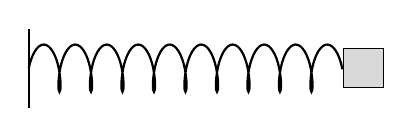
\begin{tikzpicture}
                % Dibuja la pared
                \draw[thick] (0,0.5) -- (0,1.5);

                % Dibuja el muelle
                \draw[thick, decoration={aspect=0.3, segment length=4mm, amplitude=3mm, coil}, decorate] (0,1) -- (4,1);

                % Dibuja el corcho como un cuadrado
                \draw[fill=gray!30] (4,0.75) rectangle (4.5,1.25);
            \end{tikzpicture}               
            \caption{Muelle atado a la pared.}
            \label{fig:muelle}
            \end{figure}

            De esta forma, si estiramos el muelle hacia la derecha, aparecerá una fuerza en sentido contrario. Análogamente, si comprimimos el muelle hacia la izquierda, volverá a aparecer una fuerza en sentido contrario. Se dice que la fuerza de un muelle es una fuerza recuperadora.\\

            La fórmula se deduce a partir de la Segunda Ley de Newton ($F=m\cdot a$) y de la Ley de Hooke, que nos indica que la fuerza de un muelle para una posición del cuerpo $x$ es directamente proporcional a dicha posición:
            \begin{equation*}
                F(x) = -kx
            \end{equation*}
            De esta forma:
            \begin{equation*}
                \left.\begin{array}{rl}
                    F = m\cdot a = m\cdot \ddot{x} \\
                    F(x) = -kx
            \end{array}\right\} \Longrightarrow m\ddot{x} = -kx \Longleftrightarrow m\ddot{x} + kx = 0
            \end{equation*}
            Que es una ecuación diferencial lineal de orden 2, ya que como $m\neq 0$, podemos dividir la expresión entre $m$, obteniendo que:
            \begin{equation*}
                \ddot{x} + \dfrac{k}{m}x = 0
            \end{equation*}
            Por lo que trabajamos con las funciones $a_0,a_1,b:\mathbb{R}\rightarrow\mathbb{R}$ dadas por:
            \begin{equation*}
                a_0(t) = \dfrac{k}{m} \qquad a_1(t) = 0 \qquad b(t) = 0 \qquad t\in \mathbb{R}
            \end{equation*}
        \item Como un último ejemplo de ecuación lineal que se maneja en la práctica y que es de un orden mayor que 2, en ingeniería se trabaja mucho con la ecuación que describe las vibraciones de un puente a lo largo del tiempo, que resulta en una ecuación de cuarto grado.
    \end{enumerate}
\end{ejemplo}~\\

Una vez motivado el uso e importancia de las ecuaciones lineales de orden superior, pasamos a desarrollar la teoría matemática que sustenta este tipo de ecuaciones, la cual está basada en un resultado que enunciaremos pero que se demostrará en el siguiente Capítulo (por no disponer de las herramientas necesarias por ahora).\\

Este resultado es un teorema que nos da la existencia y unicidad de una solución para cada tipo de ecuación lineal de orden $m$ (siendo $m$ cualquier número natural mayor o igual que 1), una vez fijada una condición inicial que esta función solución ha de cumplir.

\begin{definicion}[Condición inicial]
    Dada una ecuación diferencial lineal de orden $m$ cuyos coeficientes están definidos en un intervalo $I$, dar una condición inicial para dicha ecuación será dar un punto $t_0\in I$ y $m$ valores $\alpha_0,\alpha_1,\ldots,\alpha_{m-1}\in \mathbb{R}$ de forma que exijamos que para que una función $x:J\rightarrow\mathbb{R}$ (con $J\subseteq I$) sea solución de dicha ecuación, entonces ha de cumplir la condición inicial, es decir, ha de cumplir que:
    \begin{equation*}
        x(t_0) = \alpha_0, \qquad x'(t_0) = \alpha_1,\qquad  \ldots, \qquad  x^{(m-1)}(t_0) = \alpha_{m-1}
    \end{equation*}
    a parte de ser solución de dicha ecuación diferencial.
\end{definicion}~\\

De esta forma, para dar una condición inicial sobre una ecuación lineal de orden $m$, habrá que exigir $m$ ``condiciones'' sobre un mismo punto $t_0\in I$, que serán el valor de la función y de sus sucesivas derivadas (hasta la $(m-1)$-ésima) en dicho punto.

\begin{ejemplo}
    Para la ecuación del oscilador armónico:
    \begin{equation*}
        x'' + \dfrac{k}{m}x = 0
    \end{equation*}

    \begin{enumerate}
        \item Una condición inicial es exigir, por ejemplo:
            \begin{equation*}
                x(t_0) = 0 \qquad x'(t_0) = 1
            \end{equation*}

            En dicho caso, la condición inicial tiene sentido físico, ya que estaremos diciendo que en el instante $t_0$, que entendemos como el origen temporal del movimiento:
            \begin{itemize}
                \item El muelle parte del origen (posición 0) o posición de equilibrio.
                \item El muelle comienza con velocidad 1 (por lo que le hemos dado un impulso al muelle).
            \end{itemize}
            De forma intuitiva, vemos que una vez dadas una posición y velocidad iniciales al muelle, somos capaces de recrear todo el movimiento que este realizará (de forma sencilla, sabemos que el muelle se estirará y que su elasticidad ejercerá una fuerza en sentido contrario), con lo que seremos capaces de describir su posición $x$ a lo largo del tiempo $t$, con lo que para dicha condición inicial, se espera un único movimiento del muelle (una única solución de la ecuación diferencial).\\

        \item Por otra parte, la condición
            \begin{equation*}
                x(t_0) = 1 \qquad x'(t_0) = 0
            \end{equation*}
            Establece que:
            \begin{itemize}
                \item El muelle parte en la posición inicial resultado de desplazar el cuerpo conectado al muelle una unidad a la derecha (según la Figura~\ref{fig:muelle}) de la posición de equilibrio, con lo que el muelle comienza estirado.
                \item El muelle no tiene velocidad inicial.
            \end{itemize}
            En este caso, podemos pensar que una vez comience a pasar el tiempo (se vaya aumentando $t$ de forma progresiva), veremos que se ejercerá una fuerza hacia la izquierda del cuerpo, como resultado de haber estirado el muelle en un inicio, con lo que también seremos capaces de describir un único movimiento para dicho muelle en estas condiciones iniciales.
    \end{enumerate}
\end{ejemplo}

Este ejemplo nos ha servido para darnos cuenta de que, una vez fijada una condición inicial sobre un movimiento (sobre una ecuación diferencial), seremos capaces de describir la posición del móvil gracias a ese movimiento y dichas condiciones iniciales de forma única.

Por tanto, podemos ya sospechar que dar una condición inicial sobre una ecuación lineal de cualqueir orden $m$ nos es suficiente para encontrar una única solución de dicha ecuación, intuición que se manifiesta a través del siguiente teorema.

\begin{teo}[Existencia y unicidad de las soluciones]\label{teo:existencia_unicidad}
    Dada una ecuación lineal de orden $m$ cuyos coeficientes están definidos en un intervalo $I$ y dados $t_0\in I$, $\alpha_0,\alpha_1,\ldots,\alpha_{m-1}\in \mathbb{R}$ que conforman una condición inicial para dicha ecuación.

    Entonces, existe una única solución $x$ de dicha ecuación diferencial, definida en todo el intervalo $I$, que cumple las condiciones iniciales, es decir:
    \begin{equation*}
        x(t_0) = \alpha_0, \qquad x'(t_0) = \alpha_1,\qquad  \ldots, \qquad  x^{(m-1)}(t_0) = \alpha_{m-1}
    \end{equation*}

    % // TODO: Poner esto al final de la asignatura
    % \begin{proof}
        % La demostración se encuentra en el Teorema~\ref{HACER REFERENCIA}, para el cual será necesario primero repasar algunos conceptos.
    % \end{proof}
\end{teo}

Notemos que, a parte de que el teorema nos da la existencia y unicidad de las soluciones para cualquier ecuación lineal de orden $m$ (que no es poco), además nos garantiza que siempre que dicha ecuación lineal esté definida en un dominio $D=I\times J$, las soluciones estarán siempre definidas en todo el intervalo $I$, algo que no sucede con las ecuaciones diferenciales que no son lineales.

\begin{ejemplo}
    La ecuación diferencial con condición inicial:
    \begin{equation*}
        x' = x^2 \qquad x(0) = 1
    \end{equation*}

    se encuentra definida en el dominio $D=\mathbb{R}^2$, siendo sus soluciones
    \begin{equation*}
        x(t) = \dfrac{1}{1-t} \qquad t\in \left]-\infty,1\right[
    \end{equation*}

    Que no están definidas en todo $\mathbb{R}$.
\end{ejemplo}

Una vez observada la importancia de que las soluciones están definidas en todo el intervalo $I$, notemos que el Teorema~\ref{teo:existencia_unicidad} nos asegura que podemos usar las condiciones iniciales para ``etiquetar'' las soluciones de la ecuación diferencial, tal y como hacíamos en el ejemplo del muelle.\\

\begin{observacion}
    Cuando definimos una ecuación diferencial lineal de orden $m$ no tuvimos en cuenta un detalle de la definición, el cual mostraremos ahora, una vez visto el Teorema~\ref{teo:existencia_unicidad}, y es que en la definición de una ecuación lineal de orden $m$, no consideramos un coeficiente $a_m(t)$ como sí hacemos con el resto de coeficientes, sino que sólamente consideramos el caso $a_m(t) = 1$ $\forall t\in I$.\\

    Notemos que si tenemos una ecuación de la forma:
    \begin{equation*}
        a_m(t)x^{(m)} + a_{m-1}(t) x^{(m-1)} + \cdots + a_1(t)x' + a_0(t)x = b(t)
    \end{equation*}
    en la que $a_m(t) \neq 0$ $\forall t\in I$ (que para nosotros no es lineal de orden $m$), entonces podemos dividir la ecuación entera entre $a_m(t)$, obteniendo una ecuación diferencial lineal de orden $m$ con coeficientes distintos (todos ellos divididos entre $a_m$).\\

    Por tanto, este tipo de ecuaciones diferenciales no serán problema para nosotros, pero sí lo serán aquellas en las que $\exists t\in I$ tal que $a_m(t) = 0$, ya que dichas ecuaciones diferenciales no serán para nosotros ecuaciones lineales. Esto se debe a que para este tipo de ecuaciones, el Teorema~(\ref{teo:existencia_unicidad}) no es cierto, tal y como mostramos en el siguiente ejemplo.
\end{observacion}

\begin{ejemplo}
    Consideremos la ecuación diferencial
    \begin{equation*}
        tx'-x = 0
    \end{equation*}
    con dominio $D=\mathbb{R}^2$, que tiene como familia de funciones solución las rectas que pasan por el origen, tal y como vemos en la Figura~\ref{fig:familia_rectas_origen}:
    \begin{equation*}
        x(t) = ct \qquad c\in \mathbb{R}, \quad t\in \mathbb{R}
    \end{equation*}

\begin{figure}[H]
\centering    
\begin{tikzpicture}
    % Ejes coordenados
    \draw[-Stealth] (-3,0) -- (3,0) node[right] {$t$};
    \draw[-Stealth] (0,-2) -- (0,2) node[above] {$x$};

    % Dibujar las rectas para diferentes valores de c
    \draw[thick, gray!80]   (-3, -2) -- (3, 2);   % c = 1
    \draw[thick, gray!80]  (-3, -2) -- (3, 2);   % c = 0.5
    \draw[thick, gray!80] (-3, -1) -- (3, 1);   % c = 0.25
    \draw[thick, gray!80](-3, 2) -- (3, -2);   % c = -1
    \draw[thick, gray!80](-3, 2) -- (3, -2);   % c = -0.5
    \draw[thick, gray!80] (-3, 1) -- (3, -1);   % c = -0.25
\end{tikzpicture}
\caption{Familia de rectas que pasan por el origen.}
\label{fig:familia_rectas_origen}
\end{figure}
    Sin embargo, esta ecuación diferencial no es una ecuación lineal de orden 1, ya que tenemos como coeficientes $a_0,a_1,b:\mathbb{R}\rightarrow\mathbb{R}$ dados por
    \begin{equation*}
        a_0(t) = -1 \qquad a_1(t) = t \qquad b(t) = 0 \qquad t\in \mathbb{R}
    \end{equation*}
    y tenemos que $a_1(0) = 0$.\\

    Como hemos dicho anteriormente, no consideramos a este tipo de ecuaciones diferenciales como ecuaciones diferenciales lineales, y lo hacemos por una razón justificada, y es que para este tipo de ecuaciones podemos encontrar condiciones iniciales que no nos den una única solución, de forma que a veces tengamos varias soluciones para una misma condición inicial, así como que en otros casos directamente no existe una solución:

    \begin{enumerate}
        \item Si consideramos como condición inicial $x(0) = 0$, entonces tendremos infinitas soluciones de la ecuación diferencial, ya que todas las rectas de la familia anterior pasan por el punto $(0,0)$, con lo que todas ellas cumplen la ecuación inicial y son solución de la ecuación diferencial, no se cumple la unicidad.
        \item Si ahora consideramos como condición inicial $x(0)=1$, entonces no tenemos ninguna solución para la ecuación diferencial que cumpla esta condición inicial, ya que la recta vertical que pasa por el origen no forma parte de dicha familia de soluciones de la ecuación, por no ser una función. No se cumple la existencia.
    \end{enumerate}
    Por tanto, la definición de ecuación diferencial lineal va asociada al Teorema~\ref{teo:existencia_unicidad}, con lo que es otro indicador de su importancia.\\

    Sin embargo, si queremos trabajar ante este tipo de ecuaciones, como en este caso $a_1$ solo se anula en un punto, podemos considerar la ecuación lineal de orden 1:
    \begin{equation*}
        x' - \dfrac{x}{t} = 0
    \end{equation*}
    definida bien en $D^+ = \mathbb{R}^+\times \mathbb{R}$, bien en $D^- = \mathbb{R}^-\times \mathbb{R}$ y en cada caso obtenemos una ecuación lineal.

    A pesar de ello, lo que estamos haciendo es quedarnos con parte de las soluciones anteriores de forma que se cumpla la existencia y unicidad, al eliminar toda la recta $t=0$ del problema.
\end{ejemplo}~\\

\subsubsection{Ecuación lineal de orden 1}
Ya hemos comentado anteriormente que la demostración del Teorema~\ref{teo:existencia_unicidad} la dejamos para el siguiente Capítulo por no estar preparados para realizarla. Sin embargo, podemos ya demostrar un resultado más débil, que nos enuncia el teorema para el caso $m=1$:

\begin{prop}[Existencia y unicidad para ecuaciones lineales de orden 1]
    \ \\
    Dada una ecuación lineal de orden 1:
    \begin{equation*}
        x' + a_0(t)x = b(t)
    \end{equation*}
    con $a_0,b:I\rightarrow\mathbb{R}$ funciones continuas en un intervalo $I$ y dados $t_0\in I$, $\alpha_0\in \mathbb{R}$.

    Entonces, existe una única solución $x$ de la ecución lineal, definida en todo el intervalo $I$ que cumple la condición inicial, es decir:
    \begin{equation*}
        x(t_0) = \alpha_0 
    \end{equation*}
    
    \begin{proof}
        Necesitamos pues, demostrar la existencia y unicidad de dicha solución $x$:
        \begin{description}
            \item [Existencia.]~\\
                Veamos que el problema de valores iniciales
                \begin{equation*}
                    x' + a_0(t)x = b(t) \qquad x(t_0) = \alpha_0
                \end{equation*}
                tiene una solución $x$ que cumple las propiedades enuncidas. Sea pues $x:I\rightarrow\mathbb{R}$ una función dada por:
                \begin{equation*}
                    x(t) = e^{-A_0(t)} [\alpha_0 + F(t)] \qquad t\in I
                \end{equation*}

                donde $A_0,F:I\rightarrow\mathbb{R}$ son funciones definidas por
                \begin{equation*}
                    A_0(t) = \int_{t_0}^{t} a_0(s)~ds \qquad F(t) = \int_{t_0}^{t} e^{A_0(s)}b(s)~ds  \qquad t\in I
                \end{equation*}

                las cuales están bien definidas gracias al Teorema Fundamental del Cálculo, por ser $a_0$ y $e^{A_0}b$ funciones continuas en $I$ (la segunda por ser producto de una función continua por una composición de funciones continuas), con lo que $x$ está bien definida.

                Además, el Teorema Fundamental del Cálculo nos garantiza que $A_0,F\in C^1(I)$, con lo que $x\in C^1(I)$. Veamos que $x$ cumple la condición inicial y que es solución de la ecuación lineal de orden 1:

                \begin{itemize}
                    \item Por una parte, calculamos el valor de $x(t_0)$, teniendo en cuenta que:
                        \begin{align*}
                            A_0(t_0) &= \int_{t_0}^{t_0} a_0(s)~ds  = 0 \\
                            F(t_0) &= \int_{t_0}^{t_0} e^{A_0(s)}b(s)~ds = 0
                        \end{align*}

                        con lo que:
                        \begin{equation*}
                            x(t_0) = e^{-A_0(t_0)}(\alpha_0 + F(t_0)) = e^0 (\alpha_0 + 0) = \alpha_0
                        \end{equation*}
                    \item Por otra, parte, derivamos $x$ para comprobar si cumple con la ecuación diferencial, usando para ello la derivada del producto:
                        \begin{equation*}
                            x'(t) = -a_0(t)e^{-A_0(t)} [\alpha_0 + F(t)] + e^{-A_0(t)}e^{A_0(t)}b(t) \AstIg -a_0(t) x(t) + b(t)
                        \end{equation*}
                        Donde en $(\ast)$ hemos aplicado que:
                        \begin{equation*}
                            x(t) = e^{-A_0(t)} [\alpha_0 + F(t)]
                        \end{equation*}
                \end{itemize}
                Notemos que para que $x$ fuera solución era suficiente con coger como $A_0$ cualquier primitiva de $a_0$ y como $F$ cualquier primitiva de $e^{A_0}b$. Sin embargo, para que $x$ cumpliera la condición inicial, hemos tomado aquellas integrales indefinidas centradas en $t_0$.

            \item [Unicidad.]~\\
                Supongamos que tenemos dos soluciones de la ecuación lineal de orden 1 $x_1,x_2:I\rightarrow\mathbb{R}$ que cumplen con la condición inicial, es decir:
                \begin{equation*}
                    x_1(t_0) = \alpha_0 = x_2(t_0)
                \end{equation*}
                y tratamos de demostrar que dichas funciones son iguales. Para ello, definidmos $y:I\rightarrow\mathbb{R}$ dada por:
                \begin{equation*}
                    y(t) = x_1(t) - x_2(t) \qquad t\in I
                \end{equation*}

                Como $x_1,x_2$ son soluciones de la ecuación diferencial lineal, entonces son de clase $C^1(I)$, con lo que $y\in C^1(I)$ y podemos calcular su derivada:
                \begin{align*}
                    y'(t) &= x_1'(t) - x_2'(t) = -a_0(t)x_1(t) + \cancel{b(t)} + a_0(t)x_2(t) - \cancel{b(t)} \\
                          &= -a_0(t) (x_1(t) - x_2(t)) = -a_0(t)y(t) \qquad \forall t\in I
                \end{align*}
                De esta forma, si $x_1$ y $x_2$ eran soluciones de la ecuación lineal completa, resulta que $y$ es solución de la ecuación lineal homogénea asociada a dicha ecuación.\\

                Además, resulta que $y$ cumple con la condición inicial $y(t_0) = 0$:
                \begin{equation*}
                    y(t_0) = x_1(t_0) - x_2(t_0) = \alpha_0 - \alpha_0 = 0
                \end{equation*}
                Con vistas a demostrar que $y$ es constantemente igual a 0, lo que haremos será resolver la ecuación diferencial 
                \begin{equation*}
                    y' + a_0(t) y = 0
                \end{equation*}

                buscando un factor integrante para dicha ecuación. En el capítulo anterior, vimos que el factor integantes para esta ecuación era $\mu(t,x) = e^{A_0(t)}$, con lo que multiplicamos la ecuación diferencial, obteniendo que:
                \begin{equation*}
                    e^{A_0(t)}y'(t) + a_0(t)e^{A_0(t)}y(t) = 0
                \end{equation*}

                con lo que estamos ante una ecuación exacta, de forma que podemos pensar dicha expresión como la derivada de una función de una variable:
                \begin{equation*}
                    \dfrac{d}{dt}\left(e^{A_0(t)}y(t)\right) = 0
                \end{equation*}
                Como consecuencia, tenemos que las soluciones de la ecuación diferencial son de la forma:
                \begin{equation*}
                    e^{A_0(t)} y(t) = c \qquad c\in \mathbb{R} \quad t\in I
                \end{equation*}
                Sin embargo, como no buscamos todas las soluciones, sólo buscamos aquella que cumple que $y(t_0) = 0$, llegamos a que $c = 0$, con lo que la expresión de la función $y$ es:
                \begin{equation*}
                    y(t) = 0 \qquad \forall t\in I
                \end{equation*}
                Concluimos que $x_1(t) = x_2(t)$ $\forall t\in I$.
        \end{description}
    \end{proof}
\end{prop}

La demostración para el caso $m=1$ no es difícil, por lo que nos preguntamos qué es lo que hace que al pasar a cualquier $m$ esta se complique.

\subsubsection{Ecuación lineal de orden 2}
Resulta que a partir de las ecuaciones lineales de orden 2 no podemos encontrar una fórmula que nos describa las soluciones de la ecuación lineal. Veremos ahora una breve justificación de por qué no, aunque no ahondaremos mucho en el problema.

Puede demostrarse que la ecuación de Riccati (estudiada anteriormente) no tiene fórmula, así como que cualquier ecuación lineal de segundo orden puede pasarse a una ecuación de Riccati. Dada una ecuación diferencial lineal homogénea de segundo orden:

\begin{equation*}
    x'' + a_1(t) x' + a_0(t) x = 0
\end{equation*}

con $a_0,a_1:I\rightarrow\mathbb{R}$ funciones continuas en un intervalo abierto $I\subseteq \mathbb{R}$. Resulta que hay una relación entre esta ecuación y la de Riccati de 1er orden, ya que si cogemos $x:J\rightarrow\mathbb{R}$ una solución de dicha ecuación diferencial definida en un intervalo abierto $J\subseteq I$ en el que $x(t) \neq 0$ $\forall t\in J$, entonces, podemos definir $y:J\rightarrow\mathbb{R}$ dada por:
\begin{equation*}
    y(t) = \dfrac{x'(t)}{x(t)} \qquad t\in J
\end{equation*}
Que es de clase $C^1(J)$, por ser $x\in C^2(J)$ y $x(t) \neq 0$ $\forall t\in J$. Derivando:
\begin{equation*}
    y' = \dfrac{x'' x - {(x')}^{2}}{x^2}
\end{equation*}
Ahora, utilizamos que $x$ es solución de la ecuación lineal de segundo orden lineal homogénea:
\begin{equation*}
    y' = \dfrac{x'' x - {(x')}^{2}}{x^2} = \dfrac{(-a_1x' - a_0 x)x - {(x')}^{2}}{x^2} \AstIg -a_1 y - a_0 -y^2
\end{equation*}
Donde en $(\ast)$ usamos que $y = \frac{x'}{x}$. Con lo que $y$ es una función que cumple:
\begin{equation*}
    y' = -a_1(t)y - a_0(t) - y^2
\end{equation*}
Que es una ecuación de Riccati.\\

Como la ecuación de Riccati no se puede resolver en general (no tiene fórmula), podemos pensar que la ecuación lineal homogénea de segundo grado tampoco se puede resolver en general, con lo que no hay esperanza de encontrar una fórmula general.

Resulta que, conocida una solución de la ecuación lineal de segundo orden, sí que podemos encontrar sus soluciones.\\

Una ecuación lineal de tercer orden puede pasar a una de segundo orden, con lo que de esta en adelante también vemos que no hay mucha expectativa a poder hallar una fórmula para ecuaciones diferenciales lineales de orden mayor que 1, sino que el camino para resolverlas será mucho más teórico.\\

A pesar de ello, si tenemos una ecuación de la forma~(\ref{eq:linealsup}) en la que los coeficientes son funciones constantes, entonces sí que podremos hayar una fórmula para la misma, tal y como veremos próximamente.

\section{Espacio vectorial de las funciones}
Con el objetivo de desarrollar la teoría necesaria para aprender a resolver las ecuaciones diferenciales lineales, hacemos un breve repaso de álgebra lineal, viendo conceptos que ya se dieron en las asignaturas de Geometría I y Geometría II\@. Las proposiciones que carezcan de demostración se dejan como ejercicio al lector, con la finalidad de respasar dichos conceptos.

\begin{definicion}[Espacio vectorial]
    Un espacio vectorial sobre un cuerpo $\bb{K}$ es un conjunto no vacío $V$ dotado de las operaciones:
    \begin{itemize}
        \item Suma 
            \Func{+}{V\times V}{V}{(u,v)}{u+v}
        \item Producto por escalares
            \Func{\cdot}{\bb{K}\times V}{V}{(a,u)}{a\cdot u}
    \end{itemize}
    de forma que $(V,+)$ es un grupo conmutativo o abeliano y el producto por escalares cumple las propiedades:
    \begin{itemize}
        \item Pseudo-asociativa: $\qquad a\cdot (b\cdot u) = (a\cdot b)\cdot u \qquad \forall a,b\in \bb{K}, u\in V$
        \item Existencia de un elemento neutro: $\qquad \exists e\in \bb{K} \mid e\cdot u = u \qquad \forall u\in V$
        \item Distributiva respecto de la suma vectorial:
            \begin{equation*}
                a\cdot (u+v) = a\cdot u + a\cdot v \qquad \forall a\in \bb{K}, u,v\in V
            \end{equation*}
        \item Distributiva respecto de la suma escalar:
            \begin{equation*}
                (a+b)\cdot u = a\cdot u + b\cdot u \qquad \forall a,b\in \bb{K}, u\in V
            \end{equation*} 
    \end{itemize}
\end{definicion}

Repasado el concepto de espacio vectorial, en esta sección nos interesaremos por el conjunto de todas las aplicaciones sobre un intervalo abierto $I\subseteq \mathbb{R}$, por lo que definiremos el siguiente conjunto por comodidad:

\begin{definicion}
    Dado un intervalo abierto $I\subseteq \mathbb{R}$, definimos el conjunto:
    \begin{equation*}
        \bb{F}(\text{I},\mathbb{R}) = \{f:I\rightarrow\mathbb{R} \mid f \text{\ es una aplicación}\}
    \end{equation*}
\end{definicion}
Podemos pensar en $\bb{F}(\text{I}, \mathbb{R})$ también como en el conjunto de todas las curvas en explícitas.

\begin{prop}
    El conjunto $\bb{F}(I,\mathbb{R})$ junto con la suma y el producto por escalares:
    \begin{equation*}
        +:V\times V\rightarrow V \qquad \cdot:\bb{K}\times V\rightarrow V
    \end{equation*}

    dados por:
    \begin{equation*}
        \begin{array}{rcl}
            (f+g)(t) &=& f(t) + g(t) \\
            (\lm \cdot f)(t) &=& \lm \cdot (t)
        \end{array} \qquad \forall t\in I \qquad f,g\in \bb{F}(\text{I},\mathbb{R}) \quad \lm \in \mathbb{R}
    \end{equation*}
    Es un espacio vectorial sobre $\mathbb{R}$.
\end{prop}

\begin{prop}
    Dado un intervalo abierto $I\subseteq \mathbb{R}$:
    \begin{itemize}
        \item El conjunto de las funciones continuas definidas en $I$ es un subespacio vectorial de $\bb{F}(\text{I},\mathbb{R})$.
        \item El conjunto de las funciones de clase $C^k(I)$ definidas en $I$ es un subespacio vectorial de $\bb{F}(\text{I},\mathbb{R})$.
    \end{itemize}
\end{prop}

\subsection{Independencia lineal de funciones}
Repasaremos el concepto de la independencia lineal entre vectores en un espacio vectorial, concepto ya conocido pero que se manifiesta de formas distintas en relación al espacio en el que nos encontremos. Repasamos su definición:

\begin{definicion}[Independencia lineal]\ \\
    Dado un espacio vectorial $V$ sobre un cuerpo $\bb{K}$ y dados $v_1,\ldots,v_k \in V$, se dice que son linealmente independientes cuando, dados $\lm_1,\ldots,\lm_k\in \mathbb{K}$, entonces:
    \begin{equation*}
        \lm_1v_1 + \cdots + \lm_k v_k = 0 \Longrightarrow \lm_1 = \cdots = \lm_k = 0
    \end{equation*}
\end{definicion}
Es decir, que el vector 0 sólo acepta una única representación como combinacion lineal de dichos vectores.\\

En nuestro contexto, dadas $f_1,\ldots,f_k\in \bb{F}(\text{I},\mathbb{R})$, la independecia lineal de esas funciones quiere decir que, dadas $\lm_1,\ldots,\lm_k\in \mathbb{R}$ de forma que:
\begin{equation*}
    \lm_1f_1 + \cdots + \lm_k f_k = 0 
\end{equation*}

es decir, que se verifique:
\begin{equation*}
    \lm_1f_1(t) + \cdots + \lm_k f_k(t) = 0 \qquad \forall t\in I 
\end{equation*}
Entonces, tengamos que $\lm_1=\ldots=\lm_k = 0$.

\begin{definicion}[Generalización para cualquier cardinalidad]\ \\
    Dado un espacio vectorial $V$ sobre un cuerpo $\bb{K}$, sea $S\subseteq V$ un conjunto de vectores, diremos que los vectores de $S$ son linealmente independientes si, para todo subconjunto finito $F\subseteq S$, los vectores de $F$ son linealmente independientes.
\end{definicion}
Notemos que esta definición de independencia lineal para conjuntos de vectores de cualquier cardinalidad generaliza el concepto de independencia lineal para un conjunto finito de vectores, ya que siempre que tengamos $k$ vectores linealmente independientes, si nos quedamos con un subconjunto de longitud menor o igual que $k$ de dichos vectores, estos seguirán siendo linealmente independientes.\\

La independencia lineal de funciones depende del intervalo $I$, ya que podemos encontrar funciones linealmente independientes en un intervalo $J$ con $I\subsetneq J$ de forma que al restringirnos al intervalo $I$ sean linealmente dependientes (basta considerar dos funciones que coincidan en todo el intervalo $I$ y que haya algún punto de $J$ en el que no coincidan).\\

Este suceso se da porque la independencia lineal va ligada al espacio vectorial en el que nos encontremos, con lo que cuando hablemos de independencia lineal de varios vectores habrá que especificar el espacio vectorial que nos encontramos. En nuestro caso, como estaremos trabajando sobre el espacio vectorial $\bb{F}(\text{I},\mathbb{R})$, será suficiente con especificar el intervalo $I$.

\begin{prop}
    Sea $V$ un espacio vectorial sobre un cuerpo $\bb{K}$, si $S\subseteq V$ es un subespacio vectorial del mismo, dados $f_1,\ldots,f_k\in V$:
    \begin{equation*}
        f_1,\ldots,f_k \text{\ son linealmente independientes en\ } V \Longleftrightarrow \text{\ lo son en\ } S
    \end{equation*}
\end{prop}

\subsubsection{Independencia lineal por derivación}
Buscamos ahora un método para comprobar si un conjunto de funciones es linealmente independiente. Por tanto, dadas $f_1,\ldots,f_k\in \bb{F}(\text{I},\mathbb{R})$ y $\lm_1,\ldots,\lm_k\in \mathbb{R}$ de forma que:
\begin{equation*}
    \lm_1 f_1(t) + \cdots + \lm_k f_k(t) = 0 \qquad \forall t\in I
\end{equation*}
Buscamos averiguar el valor de las constantes $\lm_i$. Notemos que, si suponemos que las funciones $f_i$ son derivables al menos una vez, obtenemos que:
\begin{equation*}
    \lm_1 f_1'(t) + \cdots + \lm_k f_k'(t) = 0 \qquad \forall t\in I
\end{equation*}
Sin embargo, podemos generalizar esta igualdad, ya que si suponemos que las funciones son derivables $h$ veces para algún $h\in \mathbb{N}$, entonces:
\begin{equation*}
    \lm_1 f_1^{(h)}(t) + \cdots + \lm_k f_k^{(h)}(t) = 0 \qquad \forall t\in I
\end{equation*}
Recordemos que tratábamos de encontrar el valor de las constantes $\lm_i$. De esta forma, vemos que si suponemos que todas las funciones $f_i$ con $i \in \{1,\ldots,k\}$ son derivables $k-1$ veces, podemos encontrar $k$ ecuaciones lineales de forma que tengamos $k$ incógnitas:
\begin{equation*}
    \left\{\begin{array}{ccccccc}
            \lm_1 f_1(t) &+& \cdots &+& \lm_k f_k(t) &=& 0 \\
            \lm_1 f_1'(t) &+& \cdots &+& \lm_k f_k'(t) &=& 0 \\
            \lm_1 f_1''(t) &+& \cdots &+& \lm_k f_k''(t) &=& 0 \\
            \vdots & \vdots & \ddots & \vdots & \vdots & \vdots & \vdots \\
            \lm_1 f_1^{(k-1)}(t) &+& \cdots &+& \lm_k f_k^{(k-1)}(t) &=& 0 
    \end{array}\right.
\end{equation*}
De esta forma, no es que tengamos un sistema de ecuciones lineales que nos permita hayar el valor de los $\lm_i$, sino que tenemos un sistema de ecuaciones lineales para cada $t\in I$ con las mismas incógnitas.\\

Sin embargo, al tratarse de un sistema de ecuaciones lineal homogéneo, una solución del mismo siempre es $\lm_1=\cdots = \lm_k=0$, con lo que bastará ver que el sistema es compatible determinado para algún $t\in I$, para concluir que para dicho $t$ la solución es única, con lo que como para dicho $t$ solo sirve la solución de todos los $\lm_i$ iguales a 0, la única solución posible para todos los $t$ es esta misma.\\

En resumen, con ver que el determinante de la matriz de coeficientes del sistema para algún $t\in I$ es distinto de 0, entonces sabremos que el sistema de ecuaciones lineales superior es compatible determinado, y que una solución suya es $\lm_i=0$ $\forall i \in \{1,\ldots,k\}$, con lo que las funciones $f_1,\ldots,f_k$ eran linealmente independientes.

Con esta premisa, motivamos la siguiente definición.

\begin{definicion}[Wronskiano]\ \\
    Sea $I\subseteq \mathbb{R}$ un intervalo abierto, dadas $f_1,\ldots,f_k\in \bb{F}(\text{I},\mathbb{R})$ funciones derivables $k-1$ veces, definimos su Wronskiano como la función $W(f_1,\ldots,f_k):I\rightarrow\mathbb{R}$ dada por:
    \begin{equation*}
        W(f_1,\ldots,f_k)(t) = \left|\begin{array}{ccc}
            f_1(t) & \cdots & f_k(t) \\
            f_1'(t) & \cdots & f_k'(t) \\
            \vdots & \ddots & \vdots \\
            f_1^{(k-1)}(t) & \cdots & f_k^{(k-1)}(t) 
        \end{array}\right| \qquad t\in I
    \end{equation*}
\end{definicion}

\begin{prop}\label{prop:Wronskiano}
    Dadas $f_1,\ldots,f_k$ funciones derivables $k-1$ veces en un intervalo abierto $I$, si existe $t_0\in I$ tal que $W(f_1,\ldots,f_k)(t_0) \neq 0$. Entonces, $f_1,\ldots,f_k$ son linealmente independientes en $I$.
    \begin{proof}
        Con el desarrollo realizado hasta el momento la demostración no sería necesaria, pero la realizamos a modo de resumen.\newline
        Sean $\lm_1,\ldots,\lm_k\in \mathbb{R}$ tales que:
        \begin{equation*}
            \lm_1f_1(t) + \cdots + \lm_k f_k(t) = 0 \qquad \forall t\in I
        \end{equation*}
        Entonces, fijado $t\in I$, se cumple que:
        \begin{equation}\label{eq:sel_li}
            \left\{\begin{array}{ccccccc}
                    \lm_1 f_1(t) &+& \cdots &+& \lm_k f_k(t) &=& 0 \\
                    \lm_1 f_1'(t) &+& \cdots &+& \lm_k f_k'(t) &=& 0 \\
                    \lm_1 f_1''(t) &+& \cdots &+& \lm_k f_k''(t) &=& 0 \\
                    \vdots & \vdots & \ddots & \vdots & \vdots & \vdots & \vdots \\
                    \lm_1 f_1^{(k-1)}(t) &+& \cdots &+& \lm_k f_k^{(k-1)}(t) &=& 0 
            \end{array}\right.
        \end{equation}
        y por ser un sistema de ecuacionces lineales homogéneo, se cumple que la solución dada por $\lm_i = 0$ $\forall i \in \{1,\ldots,k\}$ es una solución del mismo (a la que llamaremos solución trivial). Como $W(f_1,\ldots,f_k)(t_0)\neq 0$, el sistema~(\ref{eq:sel_li}) es compatible determinado para dicho $t_0$, con lo que la única solución para dicho $t_0$ será la trivial.\\

        Por tanto:
        \begin{equation*}
            \lm_1f_1(t) + \cdots + \lm_k f_k(t) = 0 \quad \forall t\in I \Longrightarrow \lm_i = 0 \quad \forall i \in \{1,\ldots,k\}
        \end{equation*}
        Concluimos que $f_1,\ldots,f_k$ son linealmente independientes.
    \end{proof}
\end{prop}

\begin{ejemplo}
    Mostraremos algunos ejemplos en los que aplicaremos esta última proposición, para demostrar que ciertas aplicaciones son linealmente independientes, todos estos ejemplos trabajando sobre $\bb{F}(\mathbb{R},\mathbb{R})$.
    \begin{itemize}
        \item Consideramos las funciones seno y coseno, y veamos que estas son linealmente independientes:
            \begin{equation*}
                W(\cos, \sen)(t) = \left|\begin{array}{cc}
                    \cos(t) & \sen(t) \\
                    -\sen(t) & \cos(t) \\
                \end{array}\right| = \cos^2(t) + \sen^2(t) = 1 \neq 0
            \end{equation*}
        \item Consideramos ahora los primeros $k$ monomios: $f_0,f_1,\ldots,f_k:\mathbb{R}\rightarrow\mathbb{R}$ de forma que:
            \begin{equation*}
                f_k(t) = t^k \quad k\geq 1, \qquad f_0(t) = 1 \qquad \forall t\in \mathbb{R}
            \end{equation*}
            Veamos que $f_0,f_1,\ldots,f_k$ son linealmente independientes en $\mathbb{R}$:
            \begin{equation*}
                W(f_0,f_1,\ldots,f_k)(t) = \left|\begin{array}{ccccc}
                    1 & t & t^2 & \cdots & t^k \\
                    0 & 1 & 2t & \cdots & kt^{k-1} \\
                    0 & 0 & 2 & \cdots & k(k-1)t^{k-2} \\
                    \vdots & \vdots & \vdots & \ddots & \vdots \\
                    0 & 0 & 0 & \cdots & k!
                \end{array}\right| = 1\cdot 1\cdot 2\cdot \ldots \cdot k! \neq 0
            \end{equation*}
        \item Veamos ahora un ejemplo en el que el Wronskiano se anula en algún punto, en el caso de las funciones $f_1,f_2:\mathbb{R}\rightarrow\mathbb{R}$ dadas por $f_1(t) = \cos(t^2)$, $f_2(t) = \sen(t^2)$. Vamos a probar que son linealmente independientes en $\mathbb{R}$:
            \begin{equation*}
                W(f_1,f_2)(t) = \left|\begin{array}{cc}
                    \cos(t^2) & \sen(t^2) \\
                    -2t\sen(t^2) & 2t\cos(t^2) 
                \end{array}\right| = 2t (\cos^2(t^2) + \sen^2(t^2))= 2t
            \end{equation*}
            Por tanto, el Wronskiano se anula solo en $t=0$, pero al ser $W(f_1,f_2)(t) \neq 0$ para cualquier $t\neq 0$, sabemos gracias a la proposición anterior que $f_1$ y $f_2$ son linealmente independientes.
    \end{itemize}
\end{ejemplo}

\begin{ejemplo}
    Veamos ahora un ejemplo en el que vemos que el recíproco de la Proposición~\ref{prop:Wronskiano} es falso. Es decir, que si tenemos funciones linealmente independientes, no hay nada que impida que su Wronskiano no sea la función constantemente igual a 0. Trabjanado en $\bb{F}(\mathbb{R},\mathbb{R})$, consideramos $f_1,f_2$ las funciones dadas por:
    \begin{equation*}
        f_1(t) = t^2 \qquad f_2(t) = -|t|t \qquad t\in \mathbb{R}
    \end{equation*}
    Veamos que estas funciones son linealmente independientes en $\mathbb{R}$, pero que el Wronskiano es 0.\\

    En primer lugar, hemos de ver que $f_2$ es derivable, algo que se ve fácil si reescribimos su expresión:
    \begin{equation*}
        f_2(t) = -|t|t = \left\{\begin{array}{rr}
                -t^2 & t \geq 0 \\
                t^2 & t<0
        \end{array}\right. \qquad \forall t\in \mathbb{R}
    \end{equation*}

    luego podemos calcular su derivada:
    \begin{equation*}
        f_2'(t) = \left\{\begin{array}{rr}
                -2t & t \geq 0 \\
                2t & t \leq 0
        \end{array}\right\} = -2 |t| \qquad \forall t\in \mathbb{R}
    \end{equation*}
    Tenemos que $f_2\in C^1(\mathbb{R})$, pero que $f_2\notin C^2(\mathbb{R})$. Ya que aunque la tangente en 0 sea común, se ve que las derivadas segundas no coinciden. Estamos ya listos para calcular el Wronskiano de $f_1$ y $f_2$:
    \begin{equation*}
        W(f_1,f_2)(t) = \left|\begin{array}{cc}
            t^2  & -|t|t \\
            2t & -2|t|
        \end{array}\right| = -2|t|t^2 + 2|t|t^2 = 0 \qquad \forall t\in \mathbb{R}
    \end{equation*}
    Sin embargo, es fácil ver que son linealmente independientes, ya que $f_1$ es la parábola con vértice en el origen que diverge positivamente, mientras que $f_2$ coincide con $f_1$ en $\mathbb{R}^-$ y en $\mathbb{R}^+$ coincide con la parábola de vértice 0 que diverge negativamente, tal y como vemos en la Figura~\ref{fig:reciproco_wr}, con lo que son linealmente independientes por coincidir en un subconjunto del dominio y tener valores distintos en otro, luego no podemos encontrar $\lm\in \mathbb{R}$ tal que $f_1=\lm f_2$.
\begin{figure}[H]
\centering    
\begin{tikzpicture}
    % Ejes coordenados
    \draw[-Stealth] (-2,0) -- (2,0) node[right] {$t$};
    \draw[-Stealth] (0,-2) -- (0,2) node[above] {$x$};

    % Gráfica de f_1(t) = t^2
    \draw[blue, thick, domain=-1.4:1.4] plot (\x, {\x*\x}) node[right] {$f_1(t) = t^2$};
    
    % Gráfica de f_2(t) = -|t|t
    \draw[red, thick, domain=-1.4:1.4] plot (\x, {-abs(\x)*\x}) node[right] {$f_2(t) = -|t|t$};
\end{tikzpicture}
\caption{Gráficas de $f_1$ y $f_2$.}
\label{fig:reciproco_wr}
\end{figure}
\end{ejemplo}

\subsection{Aplicaciones lineales}\label{sec:aplicaciones_lineales}
Ahora, haremos un breve repaso de aplicaciones lineales, concepto que ya se trató en las pasadas asignaturas de Geometría o Álgebra lineal, pero que nos servirá ahora para trabajar con las ecuaciones diferenciales lineales de orden superior.
\begin{definicion}[Aplicación lineal]
    Dados $V$, $W$ espacios vectoriales sobre el mismo cuerpo $\bb{K}$, una aplicación lineal es una aplicación $L:V\rightarrow W$ de forma que:
\begin{equation*}
    L(u + v) = L(u) + L(v) \qquad L(\lm u) = \lm L(u) \qquad \forall u,v\in V, \lm \in \bb{K}
\end{equation*}
\end{definicion}
En Geometría, vimos ya que el espacio vectorial de las matrices de orden $n\cdot m$ era isomorfo al espacio vectorial de aplicaciones lineales entre espacios vectoriales de dimensiones $n$ y $m$, con lo que esencialmente, son el mismo objeto matemático.\\

Como a partir de una matriz de orden $n\cdot m$ podemos definir un único sistema de ecuaciones lineales homogéneo de $n$ ecuaciones y $m$ incógnitas, tenemos una correspondencia uno a uno entre las aplicaciones lineales y los sistemas de ecuaciones lineales.

\begin{definicion}[Núcleo]
    Dada una aplicación lineal $L:V\rightarrow W$, definimos:
    \begin{equation*}
        \ker L = \{v\in V \mid L(v) = 0\}
    \end{equation*}
\end{definicion}
Concepto que también vimos ya en Geometría, pero que ahora podemos entender como un objeto matemático que se corresponde de forma biyectiva con el conjunto de soluciones de un sistema de ecuaciones lineales, gracias a la correspondencia existente entre las aplicaciones lineales y los sistemas de ecuaciones.\\

De esta forma, cualquier tipo de ecuación (ya sea diferencial, en diferencias, \ldots) que tenga una naturaleza lineal puede ser resuelta gracias a la teoría del Álgebra lineal, como una relación de la forma:
\begin{equation*}
    L(x) = b
\end{equation*}
Para cierta aplicación lineal $L:V\rightarrow W$, siendo $x\in V$ y $b\in W$. Así, las soluciones de la ecuación de naturaleza lineal antes comentada vendrán dadas por $\ker L$.

\begin{prop}
    $\ker L$ es un subespacio vectorial de $V$.
\end{prop}
Esta última proposición nos muestra que en cualquier ecuación lineal de la naturaleza que sea, siempre que tengamos un conjunto de soluciones, este formará un espacio vectorial, con lo que la suma de soluciones también será solución y que el producto de un escalar por uan solución seguirá siendo una solución a la ecuación.

\section{Ecuación lineal homogénea de orden superior}
\noindent
Dada una ecuación diferencial lineal homogénea de cualquier orden $k$:
\begin{equation}\label{eq:linealsup_homogenea}
    x^{(k)} + a_{k-1}(t) x^{(k-1)} + \cdots + a_1(t)x' + a_0(t) x = 0
\end{equation}
con $a_0,a_1,\ldots,a_{k-1}:I\rightarrow\mathbb{R}$ funciones continuas definidas en un mismo intervalo abierto $I\subseteq \mathbb{R}$.\\

Siguiendo el último razonamiento visto en la Sección~\ref{sec:aplicaciones_lineales}, nos interesará buscar dos espacios vectoriales $V$ y $W$ sobre el mismo cuerpo $\bb{K}$, así como una aplicación lineal $L:V\rightarrow W$ de forma que seamos capaces de transformar cualquier ecuación de la forma~(\ref{eq:linealsup_homogenea}), de naturaleza lineal, en buscar una relación
\begin{equation*}
    L(x) = b \qquad x\in V \quad b\in W
\end{equation*}
de forma que el conjunto de soluciones de~(\ref{eq:linealsup_homogenea}) coincida con $\ker L$.\\

Mirando la ecuación~(\ref{eq:linealsup_homogenea}), observamos que en nuestro caso tenemos que coger una aplicación con fórmula:
\begin{equation*}
    L(x) = x^{(k)} + a_{k-1} x^{(k-1)} + \cdots + a_1x' + a_0 x 
\end{equation*}
como todas las soluciones de la ecuación serán funciones de clase $C^k(I)$, cogeremos como espacio vectorial $V=C^k(I)$, que es un espacio vectorial sobre $\mathbb{R}$, al ser subespacio de $\bb{F}(\text{I},\mathbb{R})$. Notemos que si exigimos esto sobre $x$, lo único que podemos esperar de $b$ es que sea una aplicación continua, con lo que tomamos $W = C(I)$, que también es un espacio vectorial sobre $\mathbb{R}$ por la misma razón, con lo que ya podemos definir la aplicación $L:C^k(I)\rightarrow C(I)$ dada por la fórmula superior.

\begin{definicion}[Operador diferencial]
    Dada una ecuación diferencial lineal homogénea de orden $k$ de la forma~(\ref{eq:linealsup_homogenea}), definimos su operador diferencial\footnote{``Operador'' por ser una aplicación que lleva funciones en funciones (se suele denotar con corchetes, tal y como hemos hecho) y ``diferencial'' por estar relacionado con una ecuación diferencial.} como la aplicación $L:C^k(I)\rightarrow C(I)$ dada por:
    \begin{equation*}
        L[x] = x^{(k)} + a_{k-1}x^{(k-1)} + \cdots + a_1x' + a_0x
    \end{equation*}
\end{definicion}
Es sencillo demostrar que $L$ es lineal.

\begin{ejemplo}
    Dada la ecuación
    \begin{equation*}
        x'' + t^2 x' - x = 0
    \end{equation*}
    Se trata de una ecuación lineal homogénea de orden 2, ya que podemos tomar como coeficientes las funciones $a_0,a_1:\mathbb{R}\rightarrow\mathbb{R}$ dadas por:
    \begin{equation*}
        a_1(t) = t^2, \quad a_0(t) = -1 \qquad t\in \mathbb{R}
    \end{equation*}
    El operador diferencial para esta ecuación es la función $L:C^2(\mathbb{R})\rightarrow C(\mathbb{R})$ tal que:
    \begin{equation*}
        L[x] = x'' + a_1 x' + a_0 x \qquad x\in C^2(\mathbb{R})
    \end{equation*}
    De esta forma:
    \begin{equation*}
        L[e^t] = e^t + t^2 e^t - e^t = t^2 e^t \neq 0
    \end{equation*}
    Con lo que $e^t$ no es solución de la ecuación diferencial.
\end{ejemplo}~\\

\noindent
Dada una ecuación diferencial lineal homogénea de orden $k$, podemos considerar su operador diferencial $L$, de forma que podemos tomar:
\begin{equation*}
    Z = \ker L =  \{x \in C^k(I) \mid L[x] = 0\}
\end{equation*}
Que es el conjunto de las soluciones de la ecuación lineal homogénea.

\begin{ejemplo}
    Volviendo al ejemplo de la ecuación diferencial que describe el moviemiento de un muelle:
    \begin{equation*}
        x'' + x = 0
    \end{equation*}
    Soluciones no triviales de la misma son $\varphi_1,\varphi_2:\mathbb{R}\rightarrow\mathbb{R}$ dadas por:
    \begin{equation*}
        \varphi_1(t) = \cos t, \quad \varphi_2(t) = \sen t  \qquad t\in \mathbb{R}
    \end{equation*}
    Por tanto, por ser $Z$ un espacio vectorial, todas las combinaciones lineales de $\varphi_1$ y $\varphi_2$ (recordemos que anteriormente demostramos que $\varphi_1$ y $\varphi_2$ eran linealmente independientes) son solución de dicha ecuación:
    \begin{equation*}
        \{c_1\varphi_1 + c_2\varphi_2 \mid c_1,c_2\in \mathbb{R}\} \subseteq Z
    \end{equation*}
    Nos preguntamos ahora por si hay alguna solución de la ecuación diferencial que no es combinación lineal de las funciones $\varphi_1$ y $\varphi_2$. Un primer argumento intuitivo de que sí se da la igualdad es que se trata de una ecuación lineal diferencial de segundo orden, por lo que sus soluciones dependerán de dos parámetros, y tenemos ya un espacio vectorial de dimensión 2 de soluciones de la ecuación.
\end{ejemplo}

\begin{teo}\label{teo:dim}
    Dada una ecuación diferencial lineal de orden $k$, sea $L$ su operador diferencial, consideramos $Z = \ker L$. Entonces:
    \begin{equation*}
        \dim Z = k
    \end{equation*}
    \begin{proof}
        Para ello, será suficiente con ver que existe un isomorfismo\footnote{Recordamos que un isomorfismo es una aplicación lineal biyectiva entre dos espacios vectoriales.} entre $Z$ y un espacio vectorial de dimensión $k$ sobre el mismo cuerpo. El más sencillo que se nos ocurre es $\mathbb{R}^k$. De esta forma, fijado $t_0\in I$, consideramos $\Phi_{t_0}:Z\rightarrow \mathbb{R}^k$ dada por:
        \begin{equation*}
            \Phi_{t_0}(x) = \left(x(t_0), x'(t_0), \ldots, x^{(k-1)}(t_0)\right) \qquad x\in Z
        \end{equation*}
        En primer lugar, $\Phi_{t_0}$ es lineal, ya que dados $x,y\in Z$, $\lm \in \mathbb{R}$:
        \begin{multline*}
            \Phi_{t_0}(\lm x+y) = \left(\lm x(t_0) + y(t_0), \lm x'(t_0) + y'(t_0), \ldots, \lm x^{(k-1)}(t_0) + y^{(k-1)}(t_0)\right) = \\
            =\lm \left(x(t_0), x'(t_0), \ldots, x^{(k-1)}(t_0)\right)\left(y(t_0), y'(t_0), \ldots, y^{(k-1)}(t_0)\right) = \lm \Phi_{t_0}(x) + \Phi_{t_0}(y)
        \end{multline*}

        \begin{itemize}
            \item $\Phi_{t_0}$ es un monomorfismo por la unicidad del problema de valores iniciales vista en el Teorema~\ref{teo:existencia_unicidad}, con lo que $\dim Z \leq k$.
            \item $\Phi_{t_0}$ es un epimorfismo por la existencia de las soluciones dada por el Teorema~\ref{teo:existencia_unicidad} ante una condición inicial, con lo que $\dim Z \geq k$.
        \end{itemize}
        Concluimos que $\dim Z = k$.
    \end{proof}
\end{teo}

% // TODO: Clase 19-11-24

\begin{ejemplo}
    Dada la ecuación
    \begin{equation*}
        x'' - x = 0
    \end{equation*}
    Soluciones de la misma son $\varphi_1,\varphi_2:\mathbb{R}\rightarrow\mathbb{R}$
    \begin{equation*}
        \varphi_1(t) = e^t \qquad \varphi_2(t) = e^{-t} \qquad t\in \mathbb{R}
    \end{equation*}
    Y como $\varphi_1$ y $\varphi_2$ son funciones linealmente independientes, ya que:
    \begin{equation*}
        W(\varphi_1,\varphi_2)(t) = \left|\begin{array}{cc}
            e^t & e^{-t} \\
            e^t & -e^{-t} 
        \end{array}\right| = -2  \neq 0
    \end{equation*}
    Como sabemos que el conjunto de soluciones tiene dos soluciones, sabemos que:
    \begin{equation*}
        Z = \{c_1 \varphi_1 + c_2 \varphi_2 \mid c_1,c_2 \in \mathbb{R}\}
    \end{equation*}
    Con lo que todas las soluciones de la ecuación serán de la forma:
    \begin{equation*}
        x(t) = c_1 e^t + c_2 e^{-t} \qquad c_1,c_2\in \mathbb{R} \quad t\in \mathbb{R}
    \end{equation*}
    Sin embargo, como las bases no son únicas, podemos coger también como soluciones $\psi_1,\psi_2:\mathbb{R}\rightarrow\mathbb{R}$ dadas por:
    \begin{equation*}
        \psi_1(t) = \cosh t = \dfrac{e^t + e^{-t}}{2} \qquad \psi_2(t) = \senh t = \dfrac{e^t - e^{-t}}{2} \qquad t\in \mathbb{R}
    \end{equation*}
    Que son soluciones por ser $\psi_1,\psi_2\in Z$, combinación lineal de $e^t$ y $e^{-t}$. Como también son funciones linealmente independientes (calcúlese su Wronskiano), podemos considerar:
    \begin{equation*}
        Z = \{k_1 \cosh  + k_2 \senh  \mid k_1,k_2 \in \mathbb{R}\}
    \end{equation*}
    Para esta ecuación, tenemos $\Phi_{0}:Z\rightarrow\mathbb{R}^2$ dada por:
    \begin{equation*}
        \Phi_0(x) = (x(0), x'(0)) \qquad x\in Z
    \end{equation*}

    de esta forma:
    \begin{equation*}
        \Phi_0(c_1\varphi_1 + c_2\varphi_2) = (c_1 + c_2, c_1 - c_2) \qquad \forall c_1,c_2\in \mathbb{R}
    \end{equation*}
    Respecto a la base $\{\varphi_1, \varphi_2\}$. Si ahora cambiamos la base y tomamos $\{\psi_1,\psi_2\}$, tenemos:
    \begin{equation*}
        \Phi_0(k_1\psi_1 + k_2\psi_2) = (k_1, k_2) \qquad \forall k_1,k_2\in \mathbb{R}
    \end{equation*}
    Si ahora cambiamos el punto de definición de la función, obtenemos otro isomorfismo. Por ejemplo: $\Phi_1:Z\rightarrow\mathbb{R}^2$ dada por:
    \begin{equation*}
        \Phi_1(x) = (x(1), x'(1)) \qquad x\in Z
    \end{equation*}
    Tenemos en la base $\{\varphi_1,\varphi_2\}$:
    \begin{equation*}
        \Phi_1(c_1\varphi_1+c_2\varphi_2) = \left(c_1\cdot e + \dfrac{c_2}{2}, c_1\cdot e - \dfrac{c_2}{e}\right) \qquad \forall c_1,c_2\in \mathbb{R}
    \end{equation*}

    y en la base $\{\psi_1,\psi_2\}$:
    \begin{equation*}
        \Phi_1(k_1\psi_1 + k_2\psi_2) = \left(\dfrac{k_1(e+e^{-1})+k_2(e-e^{-1})}{2}, \dfrac{k_1(e-e^{-1})+k_2(e+e^{-1})}{2}\right) \qquad \forall k_1,k_2\in \mathbb{R}
    \end{equation*}
\end{ejemplo}~\\

Con vistas a demostrar la siguiente proposición, usaremos la notación:
\begin{notacion}
    Dados $v_1,\ldots,v_k\in \mathbb{R}^k$ de forma que:
    \begin{equation*}
        v_j = (a_{1j}, a_{2j}, \ldots, a_{kj}) \qquad a_{ij}\in \mathbb{R} \quad \forall i,j\in \{1,\ldots,k\}
    \end{equation*}

    Definimos:
    \begin{equation*}
        \det(v_1|v_2|\ldots|v_k) = \det((a_{ij})_{i,j}) = \left|\begin{array}{cccc}
            a_{11} & a_{12} & \cdots & a_{1k} \\
            a_{21} & a_{22} & \cdots & a_{2k} \\
            \vdots & \vdots & \ddots & \vdots \\
            a_{k1} & a_{k2} & \cdots & a_{kk} \\
        \end{array}\right|
    \end{equation*}
\end{notacion}

\begin{prop}
    Entendiendo que estamos trabajando en relación a una ecuación diferencial lineal homogénea cuyos coeficientes están definidos en un intervalo abierto $I$, dadas $\varphi_1,\ldots,\varphi_k\in Z$, son equivalentes:
    \begin{enumerate}
        \item[$i)$] $\varphi_1,\ldots,\varphi_k$ son linealmente independientes en $I$.
        \item[$ii)$] $W(\varphi_1,\ldots,\varphi_k)(t) \neq 0$ $\forall t\in I$.
        \item[$iii)$] $\exists t_0\in I \mid W(\varphi_1,\ldots,\varphi_k)(t) \neq 0$.
    \end{enumerate}
    \begin{proof}
        Tenemos, pues, que demostrar que:
        \begin{description}
            \item [$ii)\Rightarrow iii)$] Es evidente.
            \item [$iii) \Rightarrow i)$] Por la Proposición~\ref{prop:Wronskiano}.
            \item [$i) \Rightarrow ii)$] Como $\varphi_1,\ldots,\varphi_k$ son linealmente independientes, el conjunto $\cc{B}=\{\varphi_1,\ldots,\varphi_k\}$ es una base de $Z$. Fijado $t_0\in I$, consideramos el isomorfismo $\Phi_{t_0}:Z\rightarrow\mathbb{R}^k$ definido en la demostración del Teorema~\ref{teo:dim}.

                De esta forma, el conjunto $\cc{B}'=\{\Phi_{t_0}(\varphi_1),\ldots,\Phi_{t_0}(\varphi_k)\}$ es una base de $\mathbb{R}^k$, ya que los isomorfismos llevan bases en bases.
                Como $\cc{B}'$ es una base de $\mathbb{R}^k$, entonces:
                \begin{equation*}
                    \det(\Phi_{t_0}(\varphi_1)|\ldots|\Phi_{t_0}(\varphi_k)) = W(\varphi_1,\ldots,\varphi_k)(t_0) \neq 0
                \end{equation*}
                Como $t_0$ era arbitrario, podemos repetir la demostración en cualquier $t\in I$, con lo que obtenemos que $W(\varphi_1,\ldots,\varphi_k)(t) \neq 0$ $\forall t\in I$.
        \end{description}
    \end{proof}
\end{prop}
De esta forma, entre las soluciones de una ecuación diferencial, el Wronskiano caracteriza la independencia funcional.

% // TODO: Completar
\begin{ejemplo}
    Anteriormente vimos que las funciones $f_1,f_2:\mathbb{R}\rightarrow\mathbb{R}$ dadas por:
    \begin{equation*}
        f_1(t) = \cos(t^2), \qquad f_2(t) = \sen(t^2) \qquad t\in \mathbb{R}
    \end{equation*}

    tenian como Wronskiano:
    \begin{equation*}
        W(f_1,f_2)(t) = 2t \qquad \forall t\in \mathbb{R}
    \end{equation*}
    Con lo que dichas funciones no pueden ser solución de una ecuación diferencial homogénea de segundo orden definida en todo $\mathbb{R}$.\\

    Sin embargo, es un buen ejercicio tratar de encontrar la ecuación diferencial lineal homogénea de segundo orden que verifican $f_1$ y $f_2$, con el fin de encontrar que tiene algún tipo de discontinuidad en $t=0$, con lo que probablemente solo podamos considerar dicha ecuación diferencial bien en $\mathbb{R}^+$, bien en $\mathbb{R}^-$.
\end{ejemplo}

\begin{definicion}
    Una base de $Z$ es llamada de forma clásica ``sistema fundamental''.
\end{definicion}

\subsection{Fórmula de Jacobi-Liouville}
\subsubsection{Definición de un determinante}
Antes de pasar a ver la fórmula de Jacobi-Liouville, recordaremos primero de Geometría I cuál era la definición del determinante de una matriz cuadrada, ya que necesitaremos primero ver un resultado antes de demostrar dicha fórmula.
\begin{definicion}[Permutación]
    Dado $n\in \mathbb{N}$, sea $A=\{1,\ldots,n\}$, una permutación de $A$ es cualquier aplicación biyectiva $\sigma:A\rightarrow A$.\\

    De esta forma, dado $n\in \mathbb{N}$, podemos definir el conjunto de todas las permutaciones de $\{1,\ldots,n\}$:
    \begin{equation*}
        S_n = \{\sigma \mid \sigma \text{\ es una permutación de\ } \{1,\ldots,n\}\}
    \end{equation*}
\end{definicion}
\begin{notacion}
Si $\sigma$ es una permutación de $\{1,\ldots,n\}$, es usual denotar a $\sigma$ por:
\begin{equation*}
    \sigma = (\sigma(1)\ \sigma(2)\ \ldots\ \sigma(n))
\end{equation*}
    
\end{notacion}

\begin{ejemplo}
    Para $n=2$, estaremos interesados en el conjunto $A=\{1,2\}$, con lo que todas las permutaciones de $A$ que podemos considerar son $f,g:A\rightarrow A$ dadas por:
    \begin{gather*}
        f(1) = 1 \qquad f(2) = 2 \\
        g(1) = 2 \qquad g(2) = 1 \\
    \end{gather*}
    Usando la notación anterior, tenemos que:
    \begin{align*}
        f &= (f(1)\ f(2)) = (1\ 2) \\
        g &= (g(1)\ g(2)) = (2\ 1)
    \end{align*}

    Con lo que:
    \begin{equation*}
        S_2 = \{(1\ 2),(2\ 1)\}
    \end{equation*}
\end{ejemplo}

\begin{prop}[Grupo de permutaciones]
    Se verifica que $(S_n,\circ)$ es un grupo.
\end{prop}

\begin{definicion}[Signatura]
    Sea $n\in \mathbb{N}$ y sea $\sigma\in S_n$, decimos que $\sigma$ es par si a partir de $\sigma$ podemos obtener la permutación identidad con un número par de trasposiciones (esto es, intercambiar símbolos contiguos de dicha permutación). En caso contrario, diremos que $\sigma$ es impar.\\

    \noindent
    A partir de esta definición, podemos definir la aplicación signatura, ${\veps:S_n\rightarrow\{-1,+1\}}$ dada por:
    \begin{equation*}
        \veps(\sigma) = \left\{\begin{array}{rl}
                +1 & \text{\ Si\ } \sigma \text{\ es par} \\
                -1 & \text{\ Si\ } \sigma \text{\ es impar} \\
        \end{array}\right.
    \end{equation*}
\end{definicion}

\begin{ejemplo}
    Dada la permutación de $S_5$:
    \begin{equation*}
        \sigma = (3\ 4\ 2\ 1\ 5)
    \end{equation*}
    Para obtener la permutación identidad tenemos que realizar las trasposiciones:
    \begin{enumerate}
        \item Intercambiar el 4 con el 2: $(3\ 2\ 4\ 1\ 5)$.
        \item Intercambiar el 4 con el 1: $(3\ 2\ 1\ 4\ 5)$.
        \item Intercambiar el 3 con el 2: $(2\ 3\ 1\ 4\ 5)$.
        \item Intercambiar el 3 con el 1: $(2\ 1\ 3\ 4\ 5)$.
        \item Intercambiar el 1 con el 2: $(1\ 2\ 3\ 4\ 5)$.
    \end{enumerate}
    Por lo que $\sigma$ es impar, con lo que $\veps(\sigma)=-1$.
\end{ejemplo}

\begin{definicion}
    Sea $A=(a_{ij})_{i,j} \in M_n(\bb{K})$ una matriz $n\times n$ sobre un cuerpo $\bb{K}$, definimos el determinante de $A$ como:
    \begin{equation*}
        \det(A) = \sum_{\sigma\in S_n} \veps(\sigma)\cdot  a_{1\sigma(1)}\cdot a_{2\sigma(2)}\cdot \ldots \cdot a_{n\sigma(n)}
    \end{equation*}
\end{definicion}
\begin{ejemplo}
    Para una matriz de orden 2:
    \begin{equation*}
        \left|\begin{array}{cc}
            a_{11} & a_{12} \\
            a_{21} & a_{22}
        \end{array}\right| = \sum_{\sigma\in S_2} \veps(\sigma)\cdot a_{1\sigma(1)}\cdot a_{2\sigma(2)} = a_{11}a_{22} - a_{12}a_{21}
    \end{equation*}
\end{ejemplo}

\begin{teo}[Fórmula de Jacobi-Liouville]
Dada una ecuación diferencial lineal homogénea de la forma~(\ref{eq:linealsup_homogenea}). Supongamos que tenemos $\varphi_1,\ldots,\varphi_k\in Z$, y tomamos $t_0\in I$. Entonces:
\begin{equation*}
    W(\varphi_1,\ldots,\varphi_k)(t) = W(\varphi_1,\ldots,\varphi_k)(t_0) \cdot e^{\displaystyle-\int_{t_0}^{t} a_{k-1}(s)~ds } \qquad \forall t\in I
\end{equation*}
\end{teo}
Notemos que la fórmula de Jacobi-Liouville nos da la equivalencia entre $ii)$ y $iii)$ en la última Proposición.

\subsubsection{Derivada de un determinante}
Antes de pasar a demostrar su fórmula, debemos primero averiguar cómo se deriva una función definida a partir de un determinante.

\begin{prop}
    Dadas $\{f_{ij}\}_{i,j \in \{1,\ldots,k\}}$ funciones definidas en un intervalo abierto $I$, todas ellas derivables, si definimos $D:I\rightarrow\mathbb{R}$ dada por:
    \begin{equation*}
        D(t) = \det((f_{ij}(t))_{i,j}) = \left|\begin{array}{cccc}
            f_{11}(t) & f_{12}(t) & \cdots & f_{1k}(t) \\
            f_{21}(t) & f_{22}(t) & \cdots & f_{2k}(t) \\
            \vdots & \vdots & \ddots & \vdots \\
            f_{k1}(t) & f_{k2}(t) & \cdots & f_{kk}(t) 
        \end{array}\right| \qquad t\in I
    \end{equation*}
    Entones, $D$ es derivable, con derivada:
    \begin{equation*}
        D'(t) = \left|\begin{array}{ccc}
            f_{11}'(t) & \cdots & f_{1k}'(t) \\
            f_{21}(t) & \cdots & f_{2k}(t) \\
            \vdots & \ddots & \vdots \\
            f_{k1}(t) & \cdots & f_{kk}(t) 
        \end{array}\right| + 
        \left|\begin{array}{ccc}
            f_{11}(t) & \cdots & f_{1k}(t) \\
            f_{21}'(t) & \cdots & f_{2k}'(t) \\
            \vdots & \ddots & \vdots \\
            f_{k1}(t) & \cdots & f_{kk}(t) 
        \end{array}\right| + \cdots + 
        \left|\begin{array}{ccc}
            f_{11}(t) & \cdots & f_{1k}(t) \\
            f_{21}(t) & \cdots & f_{2k}(t) \\
            \vdots & \ddots & \vdots \\
            f_{k1}'(t) & \cdots & f_{kk}'(t) 
        \end{array}\right|
    \end{equation*}
    \begin{proof}
        A partir de la definición del determinante de una matriz cuadrada, tenemos que:
        \begin{equation*}
            D(t) = \det((f_{ij}(t))_{i,j}) = \sum_{\sigma\in S_k} \veps(\sigma) f_{1\sigma(1)}(t) f_{2\sigma(2)}(t)\ldots f_{k\sigma(k)}(t)
        \end{equation*}
        Con cada $f_{ij}$ una función derivable, por lo que $D$ es derivable, y usando que la derivada de la suma es la suma de las derivadas y la fórmula de la derivada de un producto, llegamos a que:
        \begin{multline*}
            D'(t) = \sum_{\sigma\in S_k}\veps(\sigma)(f_{1\sigma(1)}(t)f_{2\sigma(2)}(t)\ldots f_{k\sigma(k)}(t))' =\\
            = \sum_{\sigma\in S_k} \veps(\sigma) f_{1\sigma(1)}'(t) f_{2\sigma(2)}(t)\ldots f_{k\sigma(k)}(t) + \sum_{\sigma\in S_k} \veps(\sigma) f_{1\sigma(1)}(t) f_{2\sigma(2)}'(t)\ldots f_{k\sigma(k)}(t) +\\+\cdots+ \sum_{\sigma\in S_k} \veps(\sigma) f_{1\sigma(1)}(t) f_{2\sigma(2)}(t)\ldots f_{k\sigma(k)}'(t)
        \end{multline*}
        Que son cada uno de los determinantes anunciados en la proposición.
    \end{proof}
\end{prop}
Notemos que como el determinante de una matriz cuadrada coincide con el determinante de su matriz traspuesta, la proposición es cierta también derivando por columnas.\\

% // TODO: Cambiar a partir de aquí
\noindent
Estamos ya listos para realizar la demostración de la Fórmula de Jacobi-Liouville:
\begin{proof}
    Probaremos la igualdad anterior probando que las dos funciones son solución de la misma ecuación diferencial lineal homogénea con las mismas condiciones iniciales, con lo que la unicidad del Teorema~\ref{teo:existencia_unicidad} nos da la igualdad funcional.\\

    Como $\varphi_1,\ldots,\varphi_k$ son soluciones de una ecuación lineal homogénea de grado $k$, tenemos que son de clase $C^1(I)$; por lo que su Wronskiano también es una función de clase $C^1(I)$, con derivada:
    \begin{equation*}
        \dfrac{d}{dt} W(\varphi_1,\ldots,\varphi_k) = \left|\begin{array}{ccc}
            \varphi_1' & \cdots & \varphi_k' \\
            \varphi_1' & \cdots & \varphi_k' \\
            \vdots & \ddots & \vdots \\
            \varphi_2^{(k-2)} & \cdots & \varphi_k^{(k-2)} \\
            \varphi_1^{(k-1)} & \cdots & \varphi_k^{(k-1)} 
        \end{array}\right| + 
        \left|\begin{array}{ccc}
            \varphi_1 & \cdots & \varphi_k \\
            \varphi_1'' & \cdots & \varphi_k'' \\
            \vdots & \ddots & \vdots \\
            \varphi_2^{(k-2)} & \cdots & \varphi_k^{(k-2)} \\
            \varphi_1^{(k-1)} & \cdots & \varphi_k^{(k-1)} 
        \end{array}\right| + \cdots + 
        \left|\begin{array}{ccc}
            \varphi_1 & \cdots & \varphi_k \\
            \varphi_1' & \cdots & \varphi_k' \\
            \vdots & \ddots & \vdots \\
            \varphi_2^{(k-2)} & \cdots & \varphi_k^{(k-2)} \\
            \varphi_1^{(k)} & \cdots & \varphi_k^{(k)} 
        \end{array}\right| 
    \end{equation*}
    De forma que todos los determinantes son 0 (por tener dos filas iguales), salvo el último, luego:
    \begin{equation*}
        \dfrac{d}{dt}W(\varphi_1,\ldots,\varphi_k) = 
        \left|\begin{array}{ccc}
            \varphi_1 & \cdots & \varphi_k \\
            \varphi_1' & \cdots & \varphi_k' \\
            \vdots & \ddots & \vdots \\
            \varphi_2^{(k-2)} & \cdots & \varphi_k^{(k-2)} \\
            \varphi_1^{(k)} & \cdots & \varphi_k^{(k)} 
        \end{array}\right| 
    \end{equation*}
    Ahora, aplicamos que $\varphi_1,\ldots,\varphi_k$ son solución de una ecuación diferencial de la forma~(\ref{eq:linealsup_homogenea}), con lo que:
    \begin{equation*}
        \varphi_i^{(k)} = -a_{k-1}\varphi_i^{(k-1)} - \ldots -a_1 \varphi_i'- a_0\varphi_i \qquad \forall i \in \{1,\ldots,k\}
    \end{equation*}
    y podemos sustituir en la fórmula anterior, aplicando la multilinealidad del determinante:
    \begin{multline*}
        \dfrac{d}{dt}W(\varphi_1,\ldots,\varphi_k) = 
        \left|\begin{array}{ccc}
            \varphi_1 & \cdots & \varphi_k \\
            \varphi_1' & \cdots & \varphi_k' \\
            \vdots & \ddots & \vdots \\
            \varphi_1^{(k-2)} & \cdots & \varphi_k^{(k-2)} \\
            \varphi_1^{(k)} & \cdots & \varphi_k^{(k)} 
        \end{array}\right| = \\
        = -a_{k-1}\left|\begin{array}{ccc}
            \varphi_1 & \cdots & \varphi_k \\
            \varphi_1' & \cdots & \varphi_k' \\
            \vdots & \ddots & \vdots \\
            \varphi_1^{(k-2)} & \cdots & \varphi_k^{(k-2)} \\
            \varphi_1^{(k-1)} & \cdots & \varphi_k^{(k-1)} 
        \end{array}\right| - \ldots -a_1
        \cancelto{0}{\left|\begin{array}{ccc}
            \varphi_1 & \cdots & \varphi_k \\
            \varphi_1' & \cdots & \varphi_k' \\
            \vdots & \ddots & \vdots \\
            \varphi_1^{(k-2)} & \cdots & \varphi_k^{(k-2)} \\
            \varphi_1' & \cdots & \varphi_k'
        \end{array}\right|} - a_0
        \cancelto{0}{\left|\begin{array}{ccc}
            \varphi_1 & \cdots & \varphi_k \\
            \varphi_1' & \cdots & \varphi_k' \\
            \vdots & \ddots & \vdots \\
            \varphi_1^{(k-2)} & \cdots & \varphi_k^{(k-2)} \\
            \varphi_1 & \cdots & \varphi_k
        \end{array}\right|} = \\
        =-a_{k-1} \left|\begin{array}{ccc}
            \varphi_1 & \cdots & \varphi_k \\
            \varphi_1' & \cdots & \varphi_k' \\
            \vdots & \ddots & \vdots \\
            \varphi_1^{(k-2)} & \cdots & \varphi_k^{(k-2)} \\
            \varphi_1^{(k-1)} & \cdots & \varphi_k^{(k-1)} 
        \end{array}\right| = -a_{k-1} \cdot W(\varphi_1,\ldots,\varphi_k)
    \end{multline*}
    Por tanto, el Wronskiano es solución de una ecuación lineal de primer orden, que cumple la condición en $t_0$:
    \begin{equation*}
        \left\{\begin{array}{rcl}
                x' &=& -a_{k-1}(t) x \\
                x(t_0) &=& W(\varphi_1,\ldots,\varphi_k)(t_0)
        \end{array}\right.
    \end{equation*}
    Que tiene una única solución:
    \begin{equation*}
        W(\varphi_1,\ldots,\varphi_k)(t_0) e^{\displaystyle -\int_{t_0}^{t} a_{k-1}(s)~ds }
    \end{equation*}

    ya que cualquier ecuación con valor inicial:
    \begin{equation*}
        \left\{\begin{array}{rcl}
                x' &=& a(t) x \\
                x(t_0) &=& x_0
        \end{array}\right.
    \end{equation*}

    Tiene por solución:
    \begin{equation*}
        x(t) = x_0\cdot  e^{\displaystyle \int_{t_0}^{t} a(s)~ds }
    \end{equation*}
    Concluimos que
    \begin{equation*}
        W(\varphi_1,\ldots,\varphi_k)(t) = W(\varphi_1,\ldots,\varphi_k)(t_0) \cdot e^{\displaystyle - \int_{t_0}^{t} a_{k-1}(s)~ds } \qquad \forall t\in I
    \end{equation*}
    Por ser ambas funciones solución de la misma ecuación diferencial con las mismas condiciones iniciales.
\end{proof}

\subsubsection{Reducción del orden}
\noindent
Supongamos que tenemos una ecuación lineal homogénea de segundo orden:
\begin{equation*}
    x'' + a_1(t) x' + a_0(t) x = 0
\end{equation*}
Con $a_0,a_1:I\rightarrow\mathbb{R}$ funciones continuas en un intervalo abierto $I\subseteq \mathbb{R}$.
Sabemos que no es posible resolverla en general, pero veamos ahora que es posible resolverla si conocemos una solución no trivial de la misma, $\varphi_1(t)$.

Notemos que resolverla equivale a, en estas condiciones, encontrar otra solución particular no trivial de la misma, $\varphi_2$ que sea linealmente independiente con $\varphi_1$, por lo que $\{\varphi_1,\varphi_2\}$ sea un sistema fundamental para dicha ecuación.\\

Buscamos pues una función $\varphi_2$ de forma que se tenga:
\begin{equation*}
    W(\varphi_1,\varphi_2)(t) = c \cdot  e^{\displaystyle -\int_{t_0}^{t} a_{k-1}~ds }
\end{equation*}
Para cualquier $c\in \mathbb{R}$. Notemos que:
\begin{equation*}
    W(\varphi_1,\varphi_2) = \varphi_1\varphi_2' - \varphi_1' \varphi_2
\end{equation*}

\begin{ejemplo}
    Como $c$ podemos coger cualquier número. Por ejemplo, si cogemos como $\varphi_1$ aquella solución con condición inicial:
    \begin{equation*}
        \varphi_1(t_0) = 2 \qquad \varphi_1'(t_0) = 0
    \end{equation*}
    Podemos coger como $c$ cualquier número, por ejemplo $c=77$:
    \begin{equation*}
        W(\varphi_1,\varphi_2)(t_0) = \left|\begin{array}{cc}
            2 & \varphi_2(t_0)  \\
            0 & \varphi_2'(t_0) \\
        \end{array}\right| = 77
    \end{equation*}
    Y bastará buscar $\varphi_2$.
\end{ejemplo}

\begin{ejemplo}
    Dada la ecuación:
    \begin{equation*}
        t^2 x'' - 2x = 0
    \end{equation*}
    Notemos que no es una ecuación lineal diferencial homogénea de segundo orden, por tener un primer coeficiente $a_2$, por lo que trabajamos con la ecuación lineal homogénea:
    \begin{equation*}
        x'' - \dfrac{2}{t^2}x = 0 \qquad t\in \mathbb{R}^+
    \end{equation*}
    Donde hemos cogido el dominio $\mathbb{R}^+$ de forma arbitraria (podíamos haber escogido también $\mathbb{R}^-$). Observamos que una solución particular de la ecuación es:
    \begin{equation*}
        \varphi(t) = t^2 \qquad t\in \mathbb{R}^+
    \end{equation*}
    Para buscar otra, dado cualquier número (salvo 0), por ejemplo, $6\in \mathbb{R}$, buscamos una nueva solución $x$ de la ecuación diferencial que cumpla:
    \begin{equation*}
        W(x,\varphi) = 6 \cdot e^{-\displaystyle \int_{t_0}^{t} a_{1}~ds } = 6\cdot e^0 = 6
    \end{equation*}
    De esta forma:
    \begin{equation*}
        W(x,\varphi) = \left|\begin{array}{cc}
            x & \varphi \\
            x' & \varphi' 
        \end{array}\right| = 2tx - t^2 x' = 6
    \end{equation*}
    Que es una ecuación lineal completa de primer orden, que ya sabemos resolver de muchas formas. Hagámoslo mediante su factor integrante, $\nicefrac{1}{t^4}$:
    \begin{equation*}
        \dfrac{2}{t^3}x - \dfrac{1}{t^2}x' = \dfrac{6}{t^4}
    \end{equation*}
    Que es una diferencial exacta:
    \begin{equation*}
        \dfrac{d}{dt}\left(\dfrac{1}{t^2}x\right) = -\dfrac{6}{t^4}
    \end{equation*}
    Integrando:
    \begin{equation*}
        \dfrac{1}{t^2}x = \dfrac{2}{t^3}
    \end{equation*}
    De esta forma:
    \begin{equation*}
        x(t) = \dfrac{2}{t} \qquad t\in \mathbb{R}^+
    \end{equation*}
    Con lo que tenemos ya un sistema fundamental de funciones de la ecuación diferencial planteada:
    \begin{equation*}
        \{\varphi, x\} = \left\{t^2, \dfrac{2}{t}\right\}
    \end{equation*}
    Por lo que el espacio de soluciones de la ecuación está conformado por las funciones que son combinación lineal de todas ellas.
\end{ejemplo}

\section{Ecución lineal completa de orden superior}
\noindent
Ahora, estaremos interesados en las ecuaciones de la forma:
\begin{equation*}
    x^{(k)} + a_{k-1}(t) x^{(k-1)} + \cdots + a_1(t) x' + a_0(t)x = b(t)
\end{equation*}
Con $b,a_0,a_1,\ldots,a_{k-1}:I\rightarrow\mathbb{R}$ funciones continuas en un intervalo abierto $I\subseteq \mathbb{R}$.\\

Para empezar, su conjunto de funciones soluciones ya no conforman un espacio vectorial, debido a que el 0 ya no es solución. Sin embargo, las ecuaciones completas están ligadas a las homogéneas, de forma que cuando se sepa resolver su homogénea asociada (aquella con los mismos coeficientes $a_i$), se sabe resolver la completa.

\subsubsection{Punto de vista geométrico}
\noindent
Dada una aplicación lineal $L:V\rightarrow W$ entre dos espacios vectoriales, podemos encontrar las ecuaciones:
\begin{equation*}
    Lx = b \qquad Lx = 0
\end{equation*}
Siendo la primera la ecuación completa y la segunda su homogénea asociada. Notemos que el conjunto de soluciones de la segunda ecuación es $\ker L$, un espacio vectorial, mientras que el conjunto de soluciones de la primera ecuación es un espacio afín, lo que se refleja en:
\begin{equation*}
    L^{-1}(b) = x_{\ast} + \ker L
\end{equation*}
con $x_{\ast}\in L^{-1}(b)$. Es decir, cualquier solución de la ecuación completa ($L^{-1}(b)$) es una solución particular $x_\ast\in L^{-1}(b)$ más una solución de la ecuación homogénea.

\begin{ejemplo}
    Dada la ecuación lineal completa:
    \begin{equation*}
        x'' + x = t^2
    \end{equation*}
    Para buscar una solución particular, como $b$ es un polinomio de segundo grado, tratamos de buscar una solución que sea un polinomio de segundo grado:
    \begin{equation*}
        \varphi(t) = \alpha + \beta t + \gamma \qquad  \varphi''(t) = 2\gamma \qquad t\in \mathbb{R}
    \end{equation*}

    con lo que buscamos la igualdad
    \begin{equation*}
        2\gamma + \alpha + \beta t + \gamma t^2 = t^2
    \end{equation*}

    Igualando coeficiente a coeficiente:
    \begin{equation*}
        \left\{\begin{array}{rll}
                2\gamma + \alpha &=& 0 \\
                \beta &=& 0 \\
                \gamma &=& 1
        \end{array}\right\} \Longrightarrow 
        \left\{\begin{array}{rlr}
                \alpha &=& -2 \\
                \beta &=& 0 \\
                \gamma &=& 1
        \end{array}\right. 
    \end{equation*}
    Con lo que la solución particular buscada es:
    \begin{equation*}
        \varphi(t) = t^2 - 2 \qquad t\in \mathbb{R}
    \end{equation*}
    Concluimos que cualquier solución de la ecuación tiene la forma:
    \begin{equation*}
        x(t) = t^2 - 2 + c_1 \cos t + c_2 \sen t \qquad c_1,c_2\in \mathbb{R} \quad t\in \mathbb{R}
    \end{equation*}
\end{ejemplo}

\begin{prop}[Principio de superposición lineal]
Supongamos que sabemos resolver dos ecuaciones completas:
\begin{equation*}
    Lx = b_1 \qquad Lx = b_2
\end{equation*}
Con una solución particular de cada una: $x_1$ y $x_2$. Entonces, ante la ecuación:
\begin{equation*}
    Lx = c_1 b_1 + c_2 b_2 \qquad c_1,c_2\in \mathbb{R}
\end{equation*}
Una solución de la ecuación será $c_1x_1 + c_2x_2$.
\end{prop}

\begin{ejemplo}
    Si ahora tenemos:
    \begin{equation*}
        x'' + x = t^2 + 2e^t
    \end{equation*}
    Lo que hacemos es aplicar el principio de superposición lineal:
    \begin{itemize}
        \item La ecuación $x'' + x = t^2$ admite como solución particular $x_1(t) = t^2 - 2$, con $t\in \mathbb{R}$.
        \item Buscamos una solución para la ecuación $x'' + x = 2e^t$, que puede comprobarse que es $x_2(t) = \nicefrac{1}{2}\cdot e^t$, con $t\in \mathbb{R}$.
    \end{itemize}
    De esta forma, una solución particular para la ecuación anterior es:
    \begin{equation*}
        \varphi(t) = t^2 - 2 + e^t \qquad t\in \mathbb{R}
    \end{equation*}
    Y para obtener el conjunto total de soluciones, es cualquier función de la forma:
    \begin{equation*}
        x(t) = t^2 - 2 + e^t + c_1 \sen t + c_2 \cos t \qquad c_1,c_2 \in \mathbb{R} \quad t\in \mathbb{R}
    \end{equation*}
\end{ejemplo}

% // TODO: Clase
\section{Ecuación lineal con coeficientes constantes}
\noindent
Estudiaremos ahora las ecuaciones lineales homogéneas\footnote{Notemos que sabiendo resolver las ecuaciones homogéneas, ya sabemos resolver las completas.} de la forma:
\begin{equation}\label{eq:lin_homog_cte}
    x^{(k)} + a_{k-1}x^{(k-1)} + \cdots + a_1x' + a_0 x = 0
\end{equation}
con $a_0,a_1,\ldots,a_{k-1}\in \mathbb{R}$. Este tipo de ecuaciones las podemos ver de la forma:
\begin{equation*}
    L[x] = 0
\end{equation*}
Siendo $L$ el operador diferencial para dicha ecuación. Estaremos interesados en el conjunto de soluciones de dicha ecuación, que sabemos ya que es $\ker L$. Para ello, bastará con encontrar un sistema fundamental para $\ker L$, que ya sabemos que ha de estar formada por $k$ funciones linealmente independientes.\\

\noindent
Para ello, evaluaremos $L$ en funciones del tipo $e^{\lm t}$, con $\lm \in \mathbb{R}$:
\begin{equation*}
    L[e^{\lm t}] = e^{\lm t}(\lm^{k} + a_{k-1}\lm^{k-1} + \cdots + a_1 \lm + a_0) = e^{\lm t} P(\lm)
\end{equation*}
Observamos que nos queda la misma función $e^{\lm t}$ por un polinomio, que es conocido tras conocer la ecuación diferencial.

\begin{definicion}[Polinomio característico]
    Dada una ecuación lineal homogénea con coeficientes constantes de la forma~(\ref{eq:lin_homog_cte}), definimos su polinomio característico como la función $P:\mathbb{R}\rightarrow\mathbb{R}$ dada por:
    \begin{equation*}
        P(\lm) = \lm^{k} + a_{k-1}\lm^{k-1} + \cdots + a_1 \lm + a_0 \qquad \lm \in \mathbb{R}
    \end{equation*}
\end{definicion}

\begin{prop}
    Dada una ecuación lineal homogénea con coeficientes constantes de la forma~(\ref{eq:lin_homog_cte}) y sea $L$ su operador diferencial, se tiene que:
    \begin{equation*}
        e^{\lm t} \in \ker L \Longleftrightarrow \lm \text{\ es raíz del polinomio característico de la ecuación}
    \end{equation*}
    \begin{proof}
        \begin{align*}
            e^{\lm t} \in \ker L \Longleftrightarrow L[e^{\lm t}] = e^{\lm t} P(\lm) = 0 \Longleftrightarrow P(\lm) = 0
        \end{align*}
    \end{proof}
\end{prop}

\begin{ejemplo}
    Se pide resolver la ecuación
    \begin{equation*}
        x'' - 5x' + 6x = 0
    \end{equation*}
    Para ello, calcularemos su polinomio característico, la función $P:\mathbb{R}\rightarrow\mathbb{R}$ dada por:
    \begin{equation*}
        P(\lm) = \lm^2 - 5\lm + 6 \qquad \lm \in \mathbb{R}
    \end{equation*}
    Buscamos las raíces de $P$:
    \begin{equation*}
        \lm = \pm \dfrac{5\pm \sqrt{25 - 24}}{2} = \left\{\begin{array}{l}
            3 \\
            2
        \end{array}\right.
    \end{equation*}
    Con lo que podemos definir las funciones $\varphi_1,\varphi_2:\mathbb{R}\rightarrow\mathbb{R}$ dadas por
    \begin{equation*}
        \varphi_1(t) = e^{2t} \qquad \varphi_2(t) = e^{3t} \qquad t\in \mathbb{R}
    \end{equation*}
    Que son linealmente independientes, ya que:
    \begin{equation*}
        \dfrac{\varphi_2(t)}{\varphi_1(t)} = \dfrac{e^{3t}}{e^{2t}} = e^t \qquad \forall t\in \mathbb{R}
    \end{equation*}
    Con lo que no existe $k\in \mathbb{R}$ tal que $\varphi_1 = k \cdot \varphi_2$, por tanto, el sistema fundamental de la ecuación es $\{e^{2t}, e^{3t}\}$.
\end{ejemplo}

\begin{observacion}
    Sean $\lm_1,\ldots,\lm_k\in \mathbb{R}$ todos ellos distintos e $I$ un intervalo no trivial, si definimos las funciones
    \begin{equation*}
        \varphi_1(t) = e^{\lm_1 t} \qquad \varphi_2(t) = e^{\lm_2 t} \qquad \ldots \qquad \varphi_k(t) = e^{\lm_k t} \qquad t\in I
    \end{equation*}
    Tenemos que todas ellas son linealmente independientes en $C^k(I)$.
    \begin{proof}
        Sabemos que $\varphi_i \in C^\infty(I)$, para cada $i \in \{1,\ldots,k\}$:
        \begin{align*}
            W(\varphi_1,\ldots,\varphi_k)(t) &= 
            \left|\begin{array}{ccc}
                e^{\lm_1 t} & \cdots & e^{\lm_k t} \\
                \lm_1e^{\lm_1 t} & \cdots & \lm_ke^{\lm_k t} \\
                \vdots & \ddots & \vdots \\
                \lm_1^{k-1}e^{\lm_1 t} & \cdots & \lm_k^{k-1}e^{\lm_k t} 
            \end{array}\right| = e^{(\lm_1+\ldots+\lm_k)t}
            \left|\begin{array}{ccc}
                1 & \cdots & 1 \\
                \lm_1 & \cdots & \lm_k \\
                \vdots & \ddots & \vdots \\
                \lm_1^{k-1} & \cdots & \lm_k^{k-1} 
            \end{array}\right| \\
                                             &\AstIg e^{(\lm_1+\ldots+\lm_k)t} \prod_{1\leq i<j \leq k} (\lm_j-\lm_i) \neq 0 \qquad \forall t\in I
        \end{align*}
        Donde en $(\ast)$ hemos usado la fórmula del determinante del Vandermonde\footnote{Vista en Métodos Numéricos I.}.
    \end{proof}
\end{observacion}

\begin{observacion}
    Dada una ecuación lineal homogénea con coeficientes constantes de la forma~(\ref{eq:lin_homog_cte}), si su polinomio característico tiene $k$ raíces reales y distintas ${\lm_1,\ldots,\lm_k \in \mathbb{R}}$, entonces $\{e^{\lm_1 t}, e^{\lm_2 t}, \ldots, e^{\lm_k t}\}$ es un sistema fundamental para~(\ref{eq:lin_homog_cte}).
\end{observacion}

\subsection{Raíces complejas del polinomio característico}
\begin{ejemplo}
    Se pide resolver la ecuación
    \begin{equation*}
        x'' + x = 0
    \end{equation*}
    Para ello, calcularemos su polinomio característico: $p(\lm) = \lm^2 + 1$, que no tiene raíces reales, ya que sus raíces son $\pm i$.
\end{ejemplo}

% Cuando el polinomio característico de una ecuación diferencial lineal con coeficientes constantes no presenta raíces reales sino complejas.
